\documentclass[dp.tex]{subfiles}
\begin{document}
\chapter{Aplikace}

V rámci této diplomové práce byla vytvořena aplikace umožňující uživateli snadné provádění dříve zmíněných testů a analýz. Aplikace je tvořena dvěma moduly:
\begin{itemize}
\item knihovnou obstarávající analýzu textů,
\item modulem obsahujícím grafické uživatelské rozhraní -- GUI.
\end{itemize}

Oba moduly jsou naprogramovány v programovacím jazyce Java. Pro spuštění aplikace je proto potřeba nejprve nainstalovat běhové prostředí Java Virtual Machine \footnote{Dostupné z \url {https://java.com/en/download}}. Součástí přílohy této diplomové práce je CD, na kterém je mimo jiné i spustitelná verze aplikace ve formátu JAR.

Velkou výhodu Javy, jak napovídá i její motto \enq{write once, run anywhere}, je její multiplatformnost. To znamená, že v Javě napsaná aplikace bude bez úprav spustitelná na všech platformách, pro něž je dostupná Java Virtual Machine. 

\section{Architektura aplikace}

Na začátku vývoje bylo třeba zvolit architekturu budoucí aplikace. Po předešlých zkušenostech z oblasti vývoje softwaru jsem se rozhodl pro dva relativně nezávislé moduly, neboť čím je program jednodušší, tím méně je náchylný k chybám. 

Prvním z těchto modulů měla být knihovna, která bude provádět samotnou analýzu textu. Tato knihovna musela být z důvodu co nejvyšší spolehlivosti důkladně otestována. Dalšími požadavky byly:
\begin{itemize}
\item rychlost,
\item multiplatformnost,
\item snadná rozšiřitelnost (např. v rámci jiné závěrečné práce).
\end{itemize}

Druhý modul měl tuto knihovnu využívat a poskytnout k ní uživatelsky přívětivé grafické rozhraní (tzv. \acrshort{gui}). Grafické rozhraní mělo umožnit uživateli otevřít textový soubor (případně více souborů), provést na něm za pomoci modulu knihovny požadovanou analýzu a zobrazit její výsledky. Důležitým požadavkem na modul grafického rozhraní byla možnost exportu vstupních dat do souboru \acrshort{csv}. 

V rámci tohoto modulu pro mě zůstala stěžejní multiplatformnost a snadná rozšiřitelnost. Vzhledem k tomu, že cílem bylo vytvořit jednoduchý frontend, nepředpokládal jsem, že by aplikace mohla být pomalá. Od automatizovaného testování jsem upustil, počítal jsem pouze s testováním uživatelským.

Vzhledem k požadavkům (multiplatformnost obou modulů, rychlost modulu knihovny) sestávala moje prvotní představa z modulu knihovny napsaném v jazyce C (případně C++) a modulu uživatelského rozhraní napsaném v některém vyšším programovacím jazyce, přičemž jsem uvažoval zejména o interpretovaných jazycích jako Python či Ruby. 

Postupně jsem však od této idei upustil a to z následujících důvodů:
\begin{enumerate}
\item Jazyk C (resp. C++) je jazyk kompilovaný. Modul knihovny by musel být pro každou cílovou platformu zkompilován samostatně.
\item Jazyky uvažované pro vývoj modulu \acrshort{gui} (Ruby, Python, \ldots) vyžadují běhové prostředí -- interpret. Ten není standardní součástí operačního systému.
\item Rychlost vývoje:
	\begin{enumerate}
	\item Vývoj v C/C++ je obecně pomalejší oproti vývoji ve vyšším programovacím jazyce. 
	\item Předpokládal jsem, že při vývoji modulu uživatelského rozhraní nastane potřeba modul knihovny modifikovat. Každá taková změna by si vyžádala spuštění vývojového prostředí, modifikaci kódu, kompilaci.
	\end{enumerate}
\end{enumerate}

Po zavrhnutí výše popsaného návrhu jsem se rozhodl oba moduly naprogramovat v jednom jazyce. To znamenalo zvolit takový jazyk, který umožní napsat jak dostatečně rychlou a otestovatelnou knihovnu, tak vytvořit grafické uživatelské rozhraní. Ve výběru zůstaly dříve zmíněné jazyky Python a Ruby a přibyly do něj jazyky C\# (Mono) a Java.

Vzhledem ke svým zkušenostem s jednotlivými jazyky jsem se nakonec rozhodl pro implementaci v jazyce Java, který splnil veškeré požadavky. 

\section{Knihovna \texttt{compLing}}

Modul knihovny jsem pojmenoval \enquote{compLing}. Název vychází z anglického \enquote{\textbf{comp}utational \textbf{ling}uistics}, což je označení pro matematickou lingvistiku. Knihovna umožňuje provádět výše zmíněné analýzy textu. 

\sloppy
K vytvoření objektu knihovny se používá statická metoda \texttt{ CompLing\#getInstance(String)}, jejímž parametrem je text, který má být analyzován. Tento text nesmí mít hodnotu \texttt{null}. Třída \texttt{CompLing} obsahuje dvě vnitřní třídy:
\begin{enumerate}
	\item \texttt{GeneralAnalysis},
	\item \texttt{PoemAnalysis}.
\end{enumerate}

Tyto třídy zapouzdřují příbuzné typy analýz. Třída \texttt{GeneralAnalysis} poskytuje přístup k analýze četnosti znaků (metodou \texttt{ICharacterFrequency characterFrequency()}) a slov (metodou \texttt{IWordFrequency wordFrequency()}). 

\sloppy
Třída \texttt{PoemAnalysis} umožňuje přístup k analýzám agregace (metoda \texttt{IAggregation aggregation()}), aliterace (metoda \texttt{IAlliteration alliteration()}), asonance (metoda \texttt{IAssonance assonance(String[])}) a denotační analýze (metoda \texttt{IDenotation denotationAnalysis()}).

Všechny metody mají jako návratový typ deklarovaná rozhraní. Díky tomu je možné změnit implementaci jednotlivých analýz bez toho, aby se změnilo \acrshort{api} knihovny. Stejně tak implementace jednotlivých analýz jsou deklarovány jako objekty implementující příslušné rozhraní. Obojí je viditelné na následujícím diagramu tříd:

\begin{figure}[h!]
	\centering
	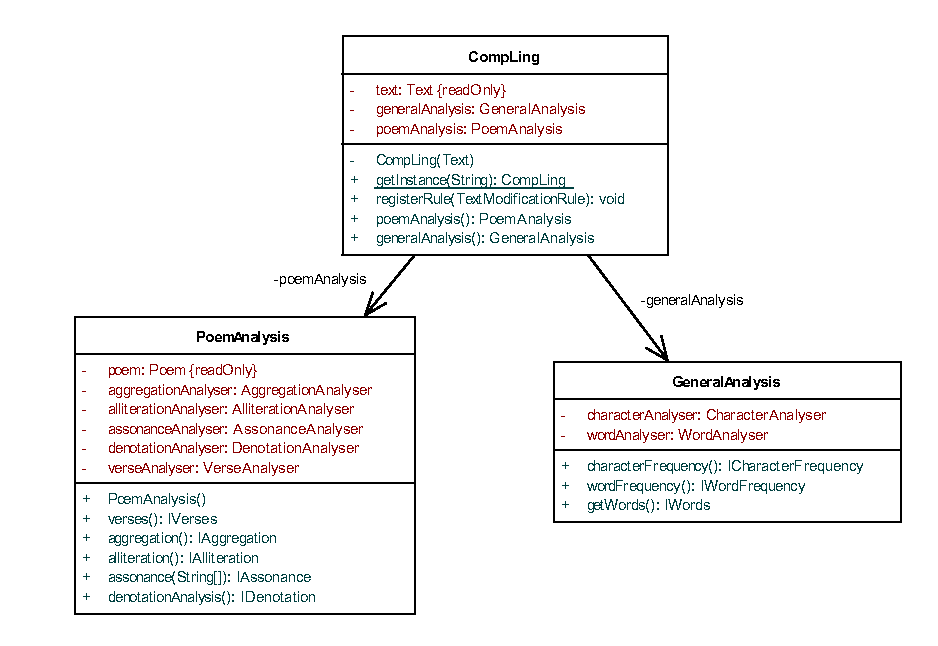
\includegraphics[width=\textwidth,keepaspectratio=true]{imgs-60-aplikace/compLing-class-diagram.pdf}
	\caption{Diagram tříd jádra knihovny \texttt{compLing}.}
\end{figure}

\section{Grafické uživatelské rozhraní}

Modul grafického uživatelského rozhraní vznikl jako nutná nadstavba nad knihovnou \texttt{compLing}, neboť knihovna sama neposkytuje žádnou jinou možnost použití (např. pomocí příkazové řádky) než \acrshort{api} a je tedy nutné začlenit ji do jiného softwarového modulu.

Cílem bylo vytvořit co možná nejjednodušší rozhraní, které uživateli umožní otevřít libovolný počet textů a následně nad těmito texty provádět analýzy podporované knihovnou \texttt{compLing}. Uživatelské rozhraní programu s 18 otevřenými překlady básně Havran je zobrazeno na následujícím obrázku:

\begin{figure}[H]
	\centering
	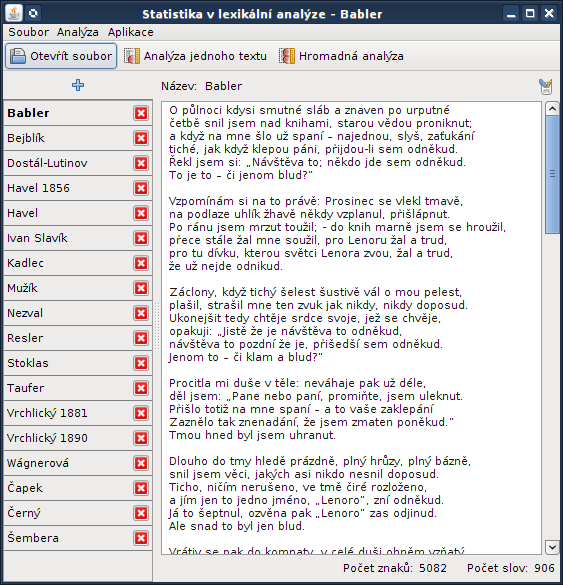
\includegraphics[max width=\textwidth,keepaspectratio=true]{imgs-60-aplikace/gui-main-window}
	\caption{Hlavní okno programu s otevřenými překlady básně Havran.}
\end{figure}

Hlavní okno je rozděleno do čtyř částí:

\begin{enumerate}
	\item menu,
	\item panel nástrojů
	\item panely otevřených textů,
	\item aktuální text.
\end{enumerate}

Menu aplikace obsahuje tři položky -- Soubor, Analýza a Aplikace. V menu Soubor se nacházejí položky pro otevření souboru a ukončení aplikace. Menu Analýza zpřístupňuje jednotlivé type analýz (kvantitativní, fonické, denotační). V případě, že není otevřen žádný text, je tato položka neaktivní. V menu Aplikace se skrývají dvě položky -- Nastavení a O aplikaci. Položka Nastavení vyvolá dialog, který umožňuje upravit velikost písma v aplikaci.

Panel nástrojů poskytuje rychlý přístup k nejčastěji využívaným funkcím. Těmi jsou otevírání textů, analýza aktuálního textu a analýza všech otevřených textů. Po kliknutí na tlačítko \enquote{Analýza jednoho textu} nebo \enquote{Hromadná analýza} je zobrazeno menu pro výběr konkrétního typu analýzy. Obě tato tlačítka jsou neaktivní, není-li otevřen žádný text.

Pod panelem nástrojů vlevo jsou ve sloupci umístěny panely pro otevřené texty. Na vrcholu panelů se nachází tlačítko pro vytvoření nového prázdného panelu. Po kliknutí pravým tlačítkem myši na panel se zobrazí kontextové menu, přes které je možné panel přejmenovat nebo uzavřít.

Nalevo od těchto panelů je zobrazen právě aktivní text. Nad i pod textem jsou umístěny dva informační panely. Vrchní zobrazuje jméno aktivního textu. Kliknutím na tlačítko vpravo (ikonka tužky) je možné text přejmenovat. Na panelu umístěném pod textem je zobrazena informace o délce aktuálního textu, a to jak v počtu znaků, tak v počtu slov.



\end{document}